\documentclass[12pt]{article}

\usepackage{amsmath, amsfonts, amsthm}
\usepackage{hyperref}
\usepackage{graphicx}
\usepackage{geometry}
\geometry{
	a4paper,
 	left=24mm,
 	right=24mm,
 	top=30mm,
 	bottom=35mm
}
\usepackage{color}
\definecolor{bluekeywords}{rgb}{0.13,0.13,1}
\definecolor{greencomments}{rgb}{0,0.5,0}
\definecolor{redstrings}{rgb}{0.9,0,0}
\definecolor{cyantypes}{RGB}{0,183,235}

\usepackage{listings}
\lstdefinelanguage{FSharp}%
{morekeywords=[1]{let, new, match, with, rec, open, module, namespace, type, of, member, % 
and, for, while, true, false, in, do, begin, end, fun, function, return, yield, try, %
mutable, if, then, else, cloud, async, static, use, abstract, interface, inherit, finally },
  morekeywords=[2]{double, float, int, string, List, BigInteger},
  otherkeywords={ let!, return!, do!, yield!, use!, var, select, where, order, by },
% otherkeywords={from}
  keywordstyle=[1]\color{bluekeywords},
  keywordstyle=[2]\color{cyantypes},
  sensitive=true,
  basicstyle=\ttfamily,
	breaklines=true,
  xleftmargin=\parindent,
  aboveskip=\bigskipamount,
	tabsize=4,
  morecomment=[l][\color{greencomments}]{///},
  morecomment=[l][\color{greencomments}]{//},
  morecomment=[s][\color{greencomments}]{{(*}{*)}},
  morestring=[b]",
  showstringspaces=false,
  literate={`}{\`}1,
  stringstyle=\color{redstrings},
}
\definecolor{codegreen}{rgb}{0,0.6,0}
\definecolor{codegray}{rgb}{0.5,0.5,0.5}
\definecolor{codepurple}{rgb}{0.58,0,0.82}
\definecolor{backcolour}{rgb}{0.95,0.95,0.92}
\lstdefinestyle{mystyle}{
    backgroundcolor=\color{backcolour},   
    commentstyle=\color{codegreen},
    keywordstyle=\color{magenta},
    numberstyle=\tiny\color{codegray},
    stringstyle=\color{codepurple},
    basicstyle=\footnotesize\ttfamily,
    breakatwhitespace=false,         
    breaklines=true,                 
    captionpos=b,                    
    keepspaces=true,                 
    numbers=left,                    
    numbersep=5pt,                  
    showspaces=false,                
    showstringspaces=false,
    showtabs=false,                  
    tabsize=4
}
\lstset{style=mystyle}

\newtheorem*{question*}{Question}
\newtheorem*{modQuestion*}{Modified Question}
\newtheorem*{origQuestion*}{Original Question}
\begin{document}


\begin{center}

{\large F\# Tutorial\\} \vspace{2mm}
\textbf{\LARGE Pipe-Forward Operator}\\
\vspace{1.5mm}
{\Large\emph{\today}}

\end{center}


\section{Modified Project Euler Solutions}

\subsubsection*{\texttt{IsPrime} Function Provided}
The following function determines whether a positive integer \texttt{x} is a prime number or not. It is already provided, and we do not need to re-implment it.
\begin{lstlisting}[language=FSharp]
let IsPrime x =
    let squareRoot = x |> double |> sqrt |> int 
    if x = 1 then false
    else if x = 2 then true
    else if x % 2 = 0 then false
    else 
        [3 .. 2 .. squareRoot]
        |> List.forall (fun i -> x%i <> 0)

// val IsPrime: x:int -> bool
\end{lstlisting}

\subsection*{Question 1} 

\url{https://projecteuler.net/problem=1}

\begin{origQuestion*}
Implement a function that sums up all multiples of $3$ or $5$ in a list.
\end{origQuestion*}

\begin{lstlisting}[language=FSharp]
let SumMultiplesOf3Or5 xList =
    xList
    |> List.filter (fun x -> x % 3 = 0 || x % 5 = 0)
    |> List.sum
\end{lstlisting}
\pagebreak

\subsection*{Question 2} 
\begin{origQuestion*}
The Fibonacci sequence (starting with $1$ and $2$) looks something like:
\[
1, 2, 3, 5, 8, 13, 21, 34, 55, 89, \ldots
\]
(For example, $1 + 2 = 3, 2 + 3 = 5, 3 + 5 = 8,$ etc.)

Find the sum of all even-valued fibonacci numbers below $4$ million.
\end{origQuestion*}
\begin{enumerate}
\item We will first test whether the $41$st fibonacci number exceeds four million or not.
\begin{lstlisting}[language=FSharp]
let first40FibNumbers =
    [1 .. 40]
    |> List.scan (fun (x,y) _ -> (y, x + y)) (1,2)
// Result: [(1,2); (2,3); ......; (267914296, 433494437)]
\end{lstlisting}
And so, we only need to consider the first $40$ or $41$ Fibonacci number. (In fact, we do not even need to consider beyond the $32$th number)
\item Sum all even-valued fibonacci numbers below $4$ million.
\begin{lstlisting}[language=FSharp]
let fibSum =
    [1 .. 40]
    |> List.scan (fun (x,y) _ -> (y, x + y)) (1,2)
    |> List.map (fun (x,y) -> x)
    |> List.filter (fun x -> x % 2 = 0)
    |> List.filter (fun x -> x < 4000000)
    |> List.sum
// Result: 4613732
\end{lstlisting}
\end{enumerate}
\subsection*{Question 3} 
\subsubsection*{Exercise (Euler Project Question 3)}

\url{https://projecteuler.net/problem=3}

Please see the next section, where we approach the original Question $3$.

\begin{modQuestion*}
Write a function that takes a list of (positive) integers, and returns the largest prime number in that list.
\end{modQuestion*}

\begin{lstlisting}[language=FSharp]
let FindLargestPrime intList =
    intList
    |> List.filter (IsPrime)
    |> List.max
\end{lstlisting}

\pagebreak
\subsection*{Question 4} 
\url{https://projecteuler.net/problem=4}
\begin{origQuestion*}
A palindromic number reads the same from left-to-right or right-to-left. 

The largest palindromic number made from the product of two 2-digit numbers is $9009 = 91 \times 99$.

Find the largest palindrome made from the product of two 3-digit numbers.
\end{origQuestion*}

The following \texttt{IsPalindrome} function that is already implemented. You do not need to re-implement it.
\begin{lstlisting}[language=FSharp]
let ReverseString (xString: string) =
    new string (xString.ToCharArray() |> Array.rev)

let IsPalindrome xString =
    (ReverseString xString) = xString

let palindromeResult1 = IsPalindrome "ASDF"   
let palindromeResult2 = IsPalindrome "ABCCBA" 
// val palindromeResult1 : bool = false
// val palindromeResult2 : bool = true
\end{lstlisting}
Find the largest palindrome number which is a product of two 3-digit numbers $a \times b$, where $100 \leq a \leq 999$, and $100 \leq b \leq 999$
\begin{lstlisting}[language=FSharp]
let findProductPalindrome =
    List.allPairs [100 .. 999] [100 .. 999]
    |> List.map (fun (a,b) -> a * b)
    |> List.filter (fun product ->
        product
        |> string
        |> IsPalindrome
    )
\end{lstlisting}
\pagebreak
\subsection*{Question 5} 
\url{https://projecteuler.net/problem=5}

\begin{modQuestion*}
Given a list of integers, find the lowest common multiple (LCM) of all those numbers. (Assume no integer overflow)
\end{modQuestion*}
Remark: We are given the following GCD and LCM functions. We do not need to re-implement them.
\begin{lstlisting}[language=FSharp]
let rec gcd x y =
    if x < 0 || y < 0 then failwith "cannot accept negative numbers"
    if x > y then gcd y x
    else if x = 0 then y
    else gcd (y % x) x

let lcm a b = 
    a * b / (gcd a b)
\end{lstlisting}
Solution:
\begin{lstlisting}[language=FSharp]
let lcmOfList xList =
    xList
    |> List.fold lcm 1

let result11 = lcmOfList [1 .. 10]
// Result: 2520

let result12 = lcmOfList [2;3;4;6;8;12]
// Result: 24
\end{lstlisting}
Remark: This method will FAIL for \texttt{xList = [1 .. 20]} because of integer overflow. Please see the next section on how to handle the original question.
\pagebreak
\subsection*{Question 6} 
\url{https://projecteuler.net/problem=6}
\begin{origQuestion*}
Given a list of integers $x_1, x_2, \ldots, x_n$, write a function that calculates the following:
\[
\left(\sum_{i=1}^n x_i\right)^2 - \left(\sum_{i=1}^n {x_i}^2\right)
\]
\end{origQuestion*}
\begin{lstlisting}[language=FSharp]
let ProjectEulerProblem6 xList =
    let sumOfSquares = 
        xList
        |> List.map (fun x -> x * x)
        |> List.sum

    let sum =
        xList
        |> List.sum

    // return
    (sum * sum) - sumOfSquares
\end{lstlisting}

\begin{lstlisting}[language=FSharp]
let result13 = ProjectEulerProblem6 [1 .. 100]
\end{lstlisting}

\subsection*{Question 7} 

\url{https://projecteuler.net/problem=7}

\begin{origQuestion*}
The list of prime numbers are $2, 3, 5, 7, 11, 13, \ldots$. We can see that the $6$th prime number is $13$. 

What is the $10001$th prime number?
\end{origQuestion*}

We start with a random guess of $500000$:
\begin{enumerate}
\item \textbf{Solution part (a)}: How many prime numbers are there between $2$ and $500000$?
\begin{lstlisting}[language=FSharp]
let numberOfPrimesWithinRange =
    [2 .. 500000]
    |> List.filter (IsPrime)
    |> List.length
\end{lstlisting}
Expected answer: $41538$. 

\item \textbf{Solution part (b)}: What is the $10001$th prime number between $2$ and $500000$?

Because of $0$-based indexing, we use \texttt{(List.item 10000)} to find the $10001$th prime number (which is between $2$ to $500000$).
\begin{lstlisting}[language=FSharp]
let find10001thPrime =
    [2 .. 500000]
    |> List.filter (IsPrime)
    |> List.item 10000
\end{lstlisting}

\end{enumerate}
\subsection*{Question 8} 
\url{https://projecteuler.net/problem=8}

\begin{modQuestion*}
Given a list of digits, find four adjacent digits with the largest product. For example, in the following number:
\[
7316717653133062491922511\mathbf{9674}426574742355349194934
\]
The 4 consecutive digits that gives the largest product is $9 \times 6 \times 7 \times 4 = 9674$

(Notice that this line is the first line in the original question)
\end{modQuestion*}
\begin{lstlisting}[language=FSharp]
let digitList = 
    [7;3;1;6;7;1;7;6;5;3;1;3;3;0;6;2;4;9;1;......]

let result8 =
    digitList
    |> List.windowed 4
    |> List.map (fun x -> x, ListProduct x)
    |> List.maxBy (fun (_,product) -> product)
// val result8 : int list * int = ([9;6;7;4], 1512)
\end{lstlisting}
Please see the next section on how we approach the original question.
\pagebreak
\subsection*{Question 9} 
\url{https://projecteuler.net/problem=9}

\begin{origQuestion*}
Find the only Pythagorean triplet $a, b, c$ that satisfy:
\[
a < b < c, \hspace{1.0cm} a + b + c = 1000, \hspace{1.0cm} a^2 + b^2 = c^2
\]
\end{origQuestion*}
\begin{lstlisting}[language=FSharp]
let FindPythagoreanTriple =
    List.allPairs [1 .. 1000] [1 .. 1000]
    |> List.filter (fun (a,b) ->
        let c = 1000 - a - b
        a * a + b * b = c * c
    )
// Result: [(200, 375); (375, 200)]
\end{lstlisting}
\subsection*{Question 10} 

\subsubsection*{Exercise (Euler Project Question 10)}

\url{https://projecteuler.net/problem=10}

Please see the next section where we work with large numbers (and potential integer overflow)
\begin{modQuestion*}
Given a number $N < 200,000$, find the sum of all prime numbers between $2$ and $N$.
\end{modQuestion*}
\begin{lstlisting}[language=FSharp]
let TotalSumOfPrimeLessThan N =
    [2 .. N]
    |> List.filter (IsPrime)
    |> List.sum
\end{lstlisting}


\pagebreak
\section{Original Project Euler Solutions}
\subsection*{Question 1} 
We did not modify Question 1.
\subsection*{Question 2} 
We did not modify Question 2.
\subsection*{Question 3} 
PLEASE EDIT THIS.
\subsection*{Question 4} 
We did not modify Question 4.
\subsection*{Question 5} 
PLEASE EDIT THIS.
\subsection*{Question 6} 
We did not modify Question 6.
\subsection*{Question 7} 
We did not modify Question 7.
\subsection*{Question 8} 
PLEASE EDIT THIS.
\subsection*{Question 9} 
We did not modify Question 9.
\subsection*{Question 10} 
\url{https://projecteuler.net/problem=10}
\begin{origQuestion*}
The sum of the primes below $10$ is $2 + 3 + 5 + 7 = 17$

Find the sum of all the primes below two million $(2,000,000)$.
\end{origQuestion*}

\begin{lstlisting}[language=FSharp]
open System.Numerics

let Version2_TotalSumOfPrimeLessThan N =
    [2 .. N]
    |> List.filter (IsPrime)
    |> List.map (BigInteger)
    |> List.sum

// Remark: The code below can take 10 seconds, as this is not the most optimal algorithm.
let result17 = Version2_TotalSumOfPrimeLessThan 2000000
// Result: 142913828922
\end{lstlisting}

\pagebreak

%%%%%%%%%%%%%%%%%%%%%%%%%%%%%%%%%%%%%%%%%%%%%%%%%%%%%%%%%%%%%
\section{Fold, Scan, State}
Key concept:
\begin{enumerate}
\item The fold and scan functions are used to keep track of states.
\begin{itemize}
\item It can be considered as eliminating a lot of intermediate steps, where the number of intermediate steps may change based on the length of the list.
\item It is somewhat similar to using a mutable state, but less things to keep track of.
\end{itemize}
\end{enumerate}
\subsection{\texttt{List.fold}}
Let us look at an example:
\begin{lstlisting}[language=FSharp]
type Commands =
    | TIMES2
    | ADD1

let listOfCommands1 =
    [TIMES2; ADD1; TIMES2; TIMES2]
\end{lstlisting}
Here, \texttt{Commands} is a discriminated union (i.e. an abstract data type) that only has two different possible values. So, it is a little bit safer than using a list of strings (because strings can take on a lot of values)

\begin{lstlisting}[language=FSharp]
let ChangingFunction prevResult currentCommand =
    match currentCommand with
    | TIMES2 -> prevResult * 2
    | ADD1 -> prevResult + 1

let startingValue = 3
\end{lstlisting}
Here, \texttt{ChangingFunction} tells us how to modify a value based on the \texttt{Commands} accepted.

\begin{lstlisting}[language=FSharp]
let result1 =
    List.fold ChangingFunction startValue listOfCommands1
// val result1 : int = 28
\end{lstlisting}

\begin{center}
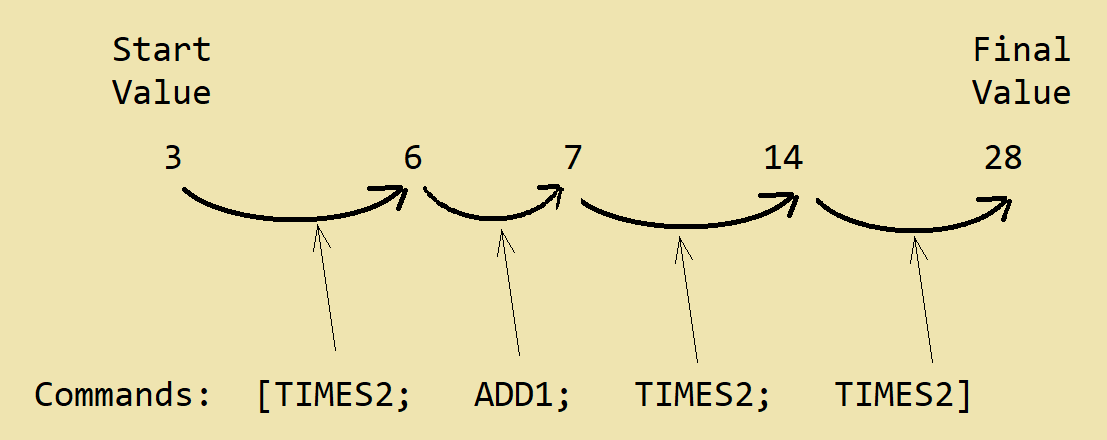
\includegraphics[width=0.8\textwidth]{pictures/picture31.png}
\end{center}
Here, we have a \texttt{startValue} of $3$, and we go through the \texttt{listOfCommands1} and evolve the \texttt{startValue} based on the \texttt{ChangingFunction}.

An equivalent implementation would be the following:

\begin{lstlisting}[language=FSharp]
let result1_version2 =
    let intermediateResult1 = 
        ChangingFunction startValue listOfCommands1.[0]

    let intermediateResult2 = 
        ChangingFunction intermediateResult1 
            listOfCommands1.[1]

    let intermediateResult3 = 
        ChangingFunction intermediateResult2 
            listOfCommands1.[2]

    let finalResult = 
        ChangingFunction intermediateResult3 
            listOfCommands1.[3]

    finalResult
\end{lstlisting}
Or if we use mutable, then:
\begin{lstlisting}[language=FSharp]
let result1_version3 =
    let mutable valueSoFar = startValue
    for command in listOfCommands1 do
        let updatedValue =
            ChangingFunction valueSoFar command
        valueSoFar <- updatedValue
    // return
    valueSoFar
\end{lstlisting}
This is most similar to codes that you may write in Java/C++

Warning: If you use VisualStudio /VisualStudioCode, you may see that \texttt{valueSoFar} is highlighted yellow in your editor, as a warning that there is a mutable value in our program. As mentioned before, F\# discourages the usage of mutable values.

\vfill

\pagebreak

\subsection{Dependance on Starting and Intermediate Value}

\subsubsection*{Dependance on Starting Value}

\begin{lstlisting}[language=FSharp]
let result1 =
    List.fold ChangingFunction startValue listOfCommands1
// val result1 : int = 28
\end{lstlisting}
\begin{center}
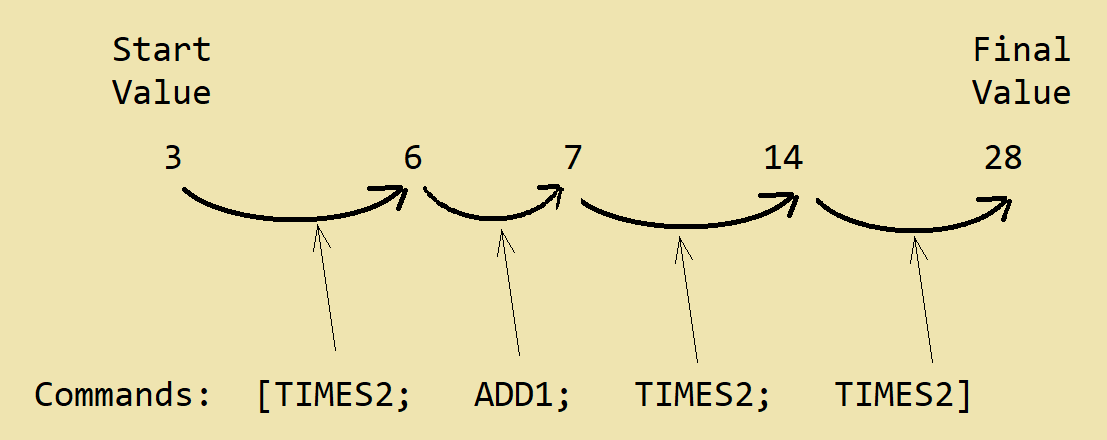
\includegraphics[width=0.8\textwidth]{pictures/picture31.png}
\end{center}
Notice that the folding process depends on the starting value:

\begin{lstlisting}[language=FSharp]
let startValue2 = 4
let result2 =
    List.fold ChangingFunction startValue2 listOfCommands1
// val result2 : int = 36
\end{lstlisting}
\begin{center}
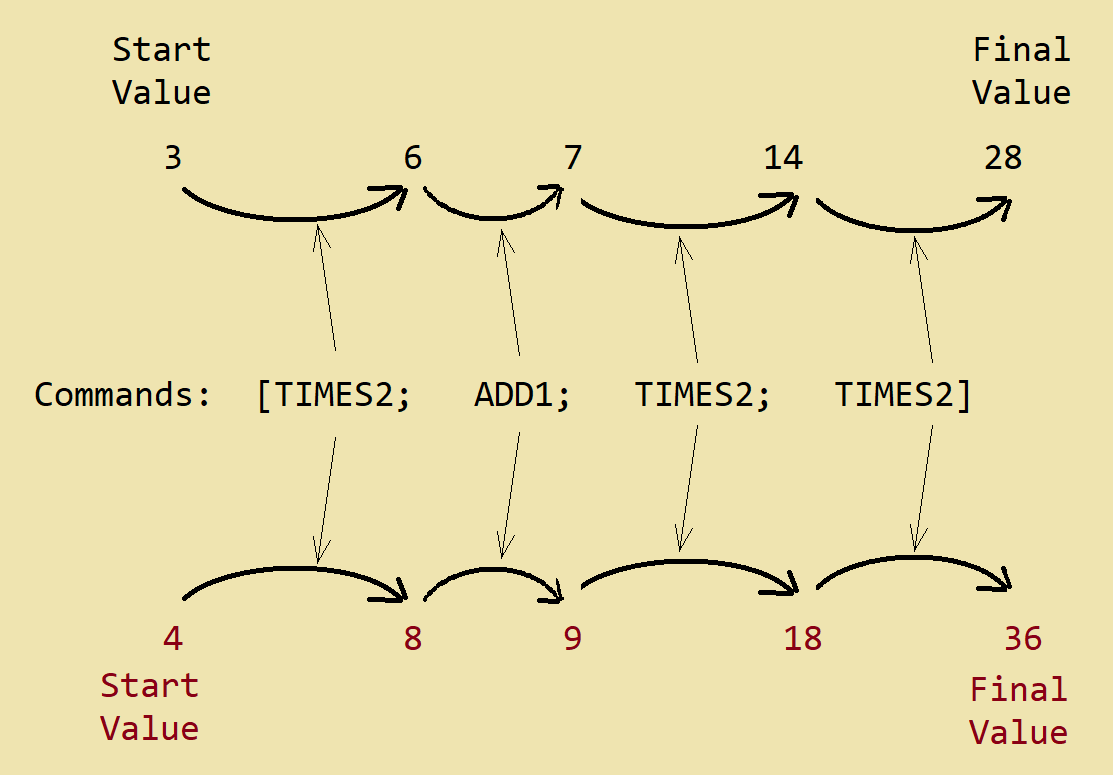
\includegraphics[width=0.8\textwidth]{pictures/picture32.png}
\end{center}

\vfill

\pagebreak

\subsubsection*{Dependance on Intermediate Value}

\begin{lstlisting}[language=FSharp]
let result1 =
    List.fold ChangingFunction startValue listOfCommands1
// val result1 : int = 28
\end{lstlisting}
\begin{center}
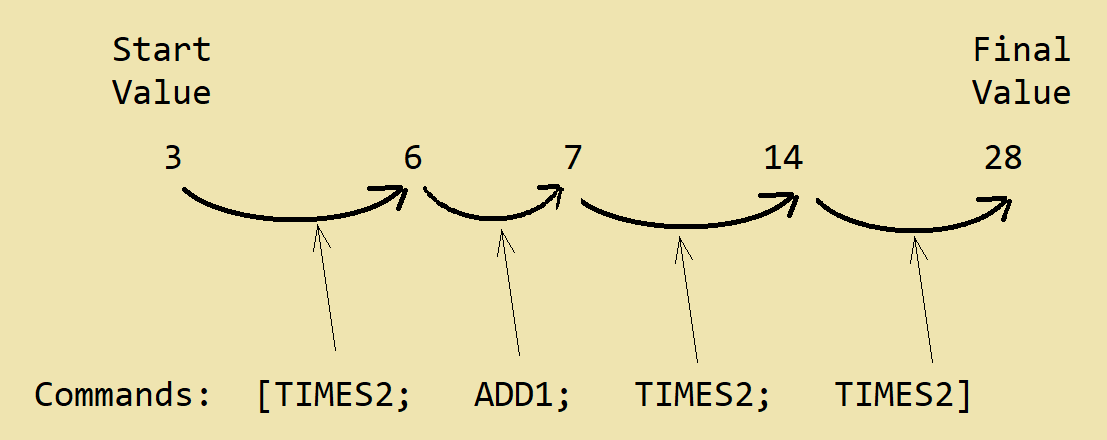
\includegraphics[width=0.8\textwidth]{pictures/picture31.png}
\end{center}
The folding process also depends on the intermediate values:

\begin{lstlisting}[language=FSharp]
let listOfCommands2 = 
    [TIMES2; ADD1; ADD1; TIMES2]

// startValue = 3

let result3 =
    List.fold ChangingFunction startValue listOfCommands2
\end{lstlisting}
\begin{center}
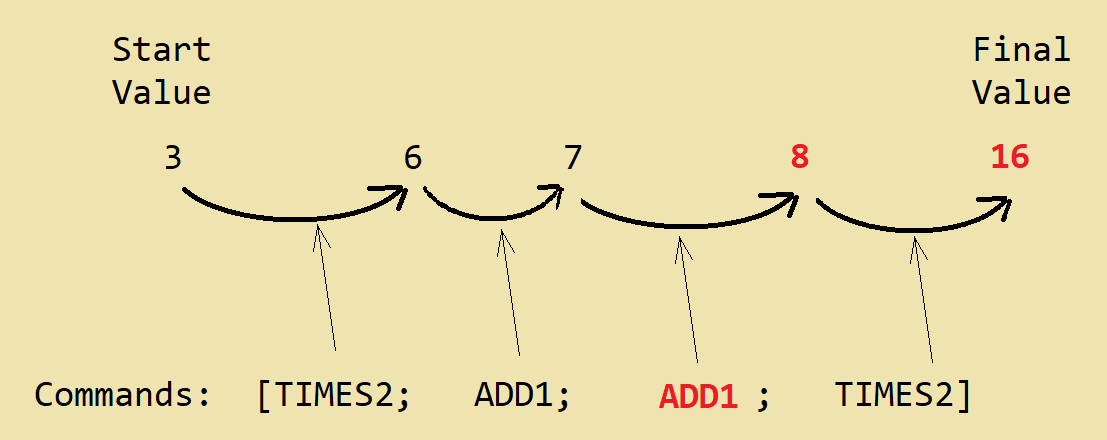
\includegraphics[width=0.8\textwidth]{pictures/picture33.png}
\end{center}

\pagebreak

\subsection{Examples}

\subsubsection*{Sum a List}

In order to sum a list, we can just use \texttt{List.sum}
\begin{lstlisting}[language=FSharp]
let result4 = List.sum [1 .. 100]
// val result4 : int = 5050
\end{lstlisting}
Alternatively, we can imagine that we are adding up the value one by one, with a starting value of $0$.

\begin{lstlisting}[language=FSharp]
let result5 = 
    [1 .. 100]
    |> List.fold (fun acc y -> acc + y) 0
// val result5 : int = 5050
\end{lstlisting}
\begin{center}
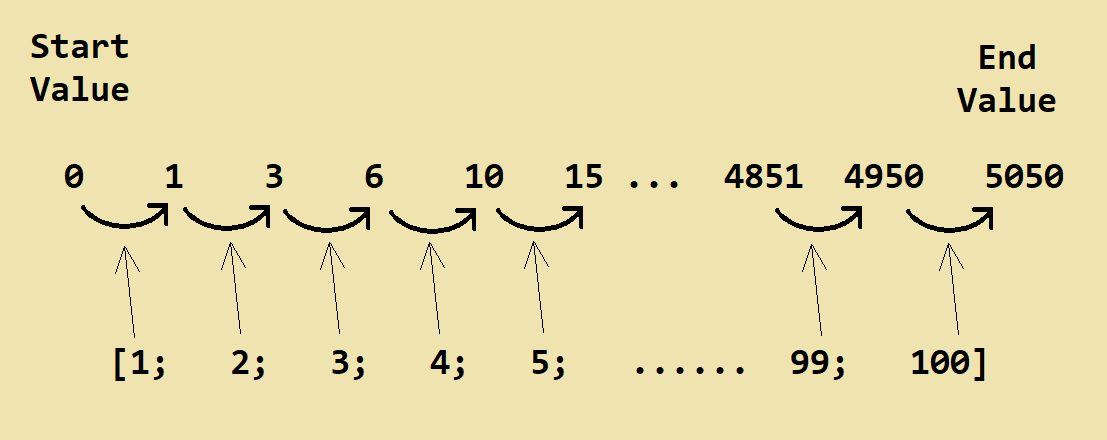
\includegraphics[width=0.8\textwidth]{pictures/picture34.png}
\end{center}
Notice that the ``folding function" is an anonymous/lambda function that accepts two variables:
\begin{itemize}
\item \texttt{acc}: The ``accumulator" or intermediate result that is used to accumulate the informations.
\item \texttt{y}: The elements from the list.
\end{itemize}
And the result of the ``folding function" is the updated ``accumulator" that will be passed on to the next accumulation stage.

If we are working in the previous case (where the accumulator is an integer, and the element of the list is a discriminated union \texttt{ADD1, TIMES2}), then it is very clear which variable is which in the anonymous function.

However, in this case of re-implementing \texttt{List.sum}, both the accumulator and the element of the list are \texttt{int}, and so we may need to be careful when we are using a non-symmetric operator, i.e:
\[
a + b =  b + a \hspace{1.0cm} a - b \neq b - a
\]

\pagebreak
\subsubsection*{Product of a List}
\begin{question*}
Write a function that takes in an integer list, and outputs the product of all elements in that list (assume no integer overflow).
\end{question*}
When you use \texttt{List.fold}, consider two things:
\begin{enumerate}
\item Which starting value should you use?
\item What does your accumulator function do? 
\end{enumerate}
\begin{lstlisting}[language=FSharp]
let ListProduct xList =
    xList
    |> List.fold (fun acc y -> ......)  .......

// What accumulating/folding function do you want to use?
// Which starting value should you use?
\end{lstlisting}
\begin{lstlisting}[language=FSharp]
let result6 = ListProduct [1 .. 5]
// Expected Result: 1 x 2 x 3 x 4 x 5 = 120

let result7 = ListProduct [2; 3; 5; 7; 11; 13]
// Expected Result: 2 x 3 x 5 x 7 x 11 x 13 = 30030
\end{lstlisting}

\vfill

\pagebreak

\subsubsection*{Application: Euler Project Question 8}

\url{https://projecteuler.net/problem=8}

\begin{modQuestion*}
Given a list of digits, find four adjacent digits with the largest product. For example, in the following number:
\[
7316717653133062491922511\mathbf{9674}426574742355349194934
\]
The 4 consecutive digits that gives the largest product is $9 \times 6 \times 7 \times 4 = 9674$

(Notice that this line is the first line in the original question)
\end{modQuestion*}
\begin{lstlisting}[language=FSharp]
let digitList = 
    [7;3;1;6;7;1;7;6;5;3;1;3;3;0;6;2;4;9;1;......]

let result8 =
    digitList
    |> List.windowed 4
    |> List.map (fun x -> x, ListProduct x)
    |> List.maxBy (fun (_,product) -> product)
// val result8 : int list * int = ([9;6;7;4], 1512)
\end{lstlisting}
We will use the picture below to illustrate what we are trying to achieve here.
\begin{center}
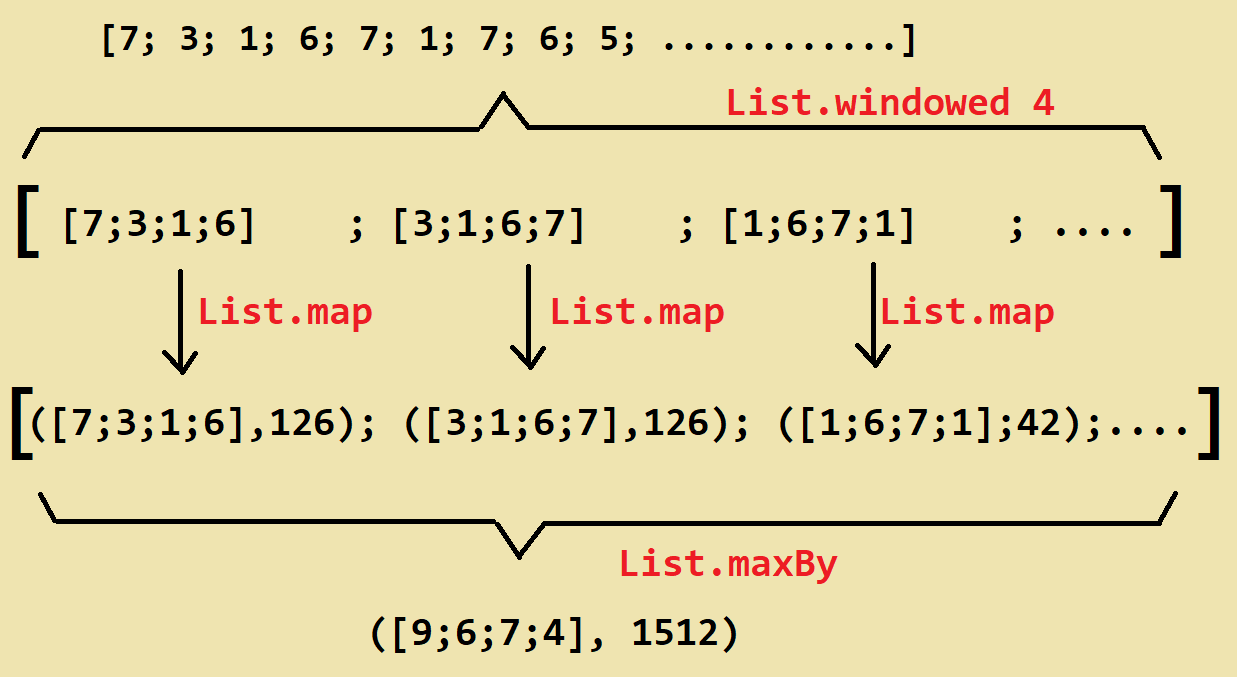
\includegraphics[width=\textwidth]{pictures/picture35.png}
\end{center}

Our goal here is to show that the \texttt{ListProduct} that we have implemented before using \texttt{List.fold} can be very powerful when combined with other \texttt{List} functions (e.g. \texttt{List.windowed}, \texttt{List.maxBy}, etc.) . To see how we approach the original Euler Problem, see the appendix. 
\pagebreak

\subsubsection*{Example: GCD of a list of integers}
\subsubsection*{GCD for two variables already provided}
You are given the following recursive \texttt{rec} function, that helps to calculate the greatest common divisor (GCD) of two integers. (This is Euclidean Algorithm)
\begin{lstlisting}[language=FSharp]
let rec gcd x y =
    if x < 0 || y < 0 then failwith "cannot accept negative numbers"
    if x > y then gcd y x
    else if x = 0 then y
    else gcd (y % x) x
\end{lstlisting}
Reminder: You do not need to re-implement this function. You can just use it.
\begin{question*}
Given a list of (positive) integers, find the greatest common divisor (GCD) of those integers.
\end{question*}
Strategy: We make the following observation:
\begin{align*}
GCD\left(x_1, x_2, x_3\right) &= GCD\left[GCD\left(x_1, x_2\right), x_3\right]
\\GCD\left(x_1, x_2, x_3, x_4\right) &= GCD\left[GCD\left(x_1, x_2, x_3\right), x_4\right]
\\ \vdots \hspace{2.0cm}&= \hspace{2.0cm} \vdots
\\GCD\left(x_1, x_2, \ldots, x_n\right) &= GCD\left[GCD\left(x_1, \ldots, x_{n-1}\right), x_n\right]
\end{align*}
\begin{lstlisting}[language=FSharp]
let gcdOfList xList =
    let first = xList |> List.head
    let remaining = xList |> List.tail

    remaining
    |> List.fold gcd first
\end{lstlisting}
We will use the picture below to illustrate what we are trying to achieve here.
\begin{center}
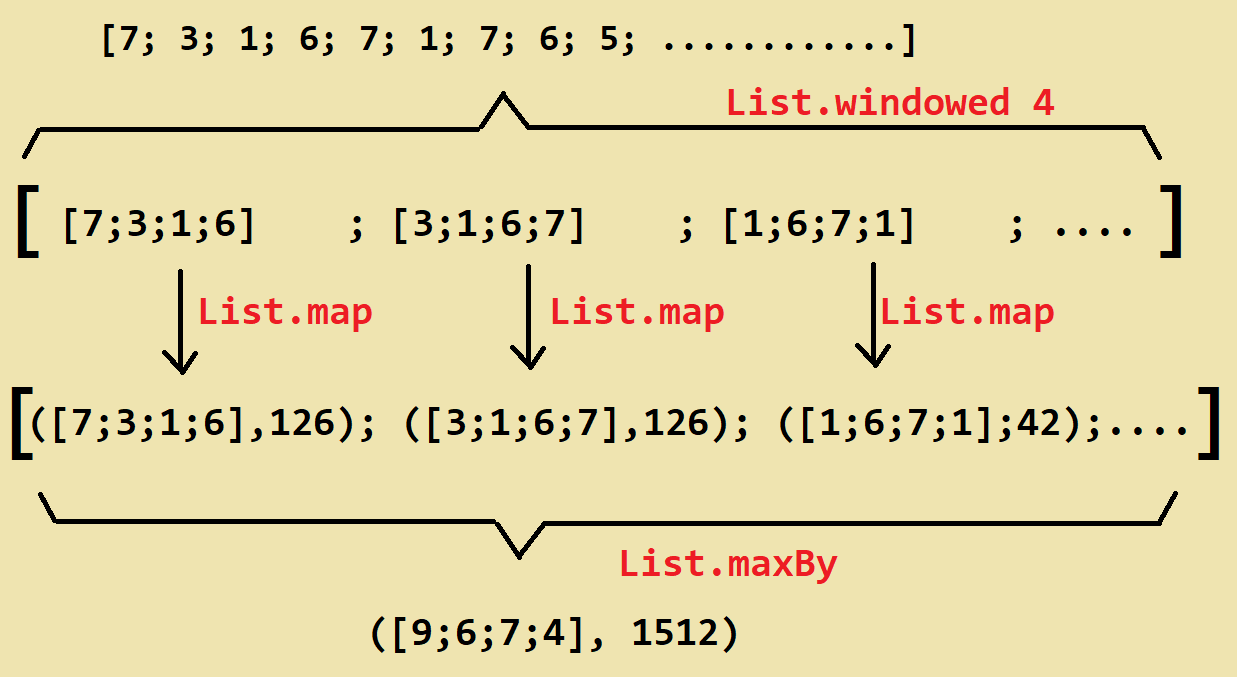
\includegraphics[width=0.2\textwidth]{pictures/picture35.png}
\end{center}

\pagebreak

\subsubsection*{Exercise: Euler Project Question 5}

\url{https://projecteuler.net/problem=5}

\begin{modQuestion*}
Given a list of integers, find the lowest common multiple (LCM) of all those numbers. (Assume no integer overflow)
\end{modQuestion*}
Strategy: We make the following observation:
\begin{align*}
LCM\left(x_1, x_2\right) &= LCM\left[LCM\left(x_1\right), x_2\right]
\\LCM\left(x_1, x_2, x_3\right) &= LCM\left[LCM\left(x_1, x_2\right), x_3\right]
\\LCM\left(x_1, x_2, x_3, x_4\right) &= LCM\left[LCM\left(x_1, x_2, x_3\right), x_4\right]
\\ \vdots \hspace{2.0cm}&= \hspace{2.0cm} \vdots
\\LCM\left(x_1, x_2, \ldots, x_n\right) &= LCM\left[LCM\left(x_1, \ldots, x_{n-1}\right), x_n\right]
\end{align*}
Hint: You can directly use the LCM function as your folding function. You do not need to re-implement it. 
\begin{lstlisting}[language=FSharp]
let lcm a b = 
    a * b / (gcd a b)
\end{lstlisting}
So, we do not need to worry about our folding function, and we just need to worry about the starting value.

\begin{lstlisting}[language=FSharp]
let lcmOfList xList =
    xList
    |> List.fold lcm ........

let result11 = lcmOfList [1 .. 10]
// Result: 2520

let result12 = lcmOfList [2;3;4;6;8;12]
// Result: 24
\end{lstlisting}

{\Large \textbf{Warning:}} If you try to use this function on the list \texttt{[1 .. 20]}, you may either see an error, or see the following wrong result:
\begin{lstlisting}[language=FSharp]
let result11 = lcmOfList [1 .. 20]
// Wrong Result: 18044195
// WRONG RESULT!!!!!!
\end{lstlisting}
Again, this is because of integer overflow (\texttt{int} cannot handle large numbers). You can see the Appendix on how to handle this situation.

\pagebreak

\subsubsection*{Exercise: Euler Project Question 2}

\pagebreak

\appendix
\section{Appendix}


\subsection{Project Euler In-Depth}

\subsubsection{Euler Project Question 3}

\url{https://projecteuler.net/problem=3}

In the main chapter, we asked you to solve a modified version of Project Euler Q3:
\begin{modQuestion*}
Write a function that takes a list of (positive) integers, and returns the largest prime number in that list.
\end{modQuestion*}
Hopefully, by using the \texttt{IsPrime} function provided in the main chapter, your answer is:
\begin{lstlisting}[language=FSharp]
let FindLargestPrime intList =
    intList
    |> List.filter (IsPrime)
    |> List.max
\end{lstlisting}

How is this related to the original question?
\begin{question*}
Given an integer $Z$, write a function that finds the largest prime factor of $Z$. e.g. The prime factors of $13195$ are $5, 7, 13, 29$, and so the largest for $13195$ is $29$.
\end{question*}

\subsubsection*{Problem Analysis}
In our ``modified approach'' in the original text, we tried to find the largest prime factor of $Z$ between $2$ and $\sqrt{Z}$. However, given an integer $Z$, it is possible that the largest prime factor of $Z$ is greater than $\sqrt{Z}$
\begin{itemize}
\item Example: $3 \times 7 = 21$. The largest prime factor is $7 > \sqrt{21} \approx 4.58$.

\item Example: $6 \times 11 = 66$. The largest prime factor is $11 > \sqrt{66} \approx 8.12$.
\end{itemize}
We will modify our approach to the following method:
\begin{enumerate}
\item Let $S_1 = \{a_1, \ldots, a_n\}$ be all the factors of $Z$ (not necessarily prime factors) between $1$ and $\sqrt{Z}$. This set will always contain at least one element: $a_1 = 1$.
\item Let $S_2 = \left\{\dfrac{Z}{a_1},\ldots, \dfrac{Z}{a_n}\right\}$. These are all the factors of $Z$ between $\sqrt{Z}$ and $Z$. This set will always contain at least one element: $\dfrac{Z}{a_1} = Z$.
\item So, $S_1 \cup S_2 =  \left\{a_1, \ldots, a_n, \dfrac{Z}{a_1},\ldots, \dfrac{Z}{a_n}\right\}$ are all the factor of $Z$ (not necessarily prime factors).
\item Out of our list of candidates $S_1 \cup S_2$, which number is the \underline{largest}, \underline{prime} number?
\end{enumerate}

\subsubsection*{Working with \texttt{BigInteger}:}
\begin{enumerate}
\item We will need an \texttt{IsPrimeBigInteger} function that helps us check whether a \texttt{BigInteger} is a prime number or not.
\begin{lstlisting}[language=FSharp]
let IsPrimeBigInteger x =
    let squareRoot = x |> double |> sqrt |> BigInteger 
    if x = BigInteger(1) then false
    else if x = BigInteger(2) then true
    else if x % BigInteger(2) = BigInteger(0) then false
    else 
        [BigInteger(3) .. BigInteger(2) .. squareRoot]
        |> List.forall (fun i -> x%i <> BigInteger(0))
\end{lstlisting}
\item When \texttt{x, y} are both \texttt{BigInteger}s, then cannot do \texttt{x \% y = 0}, because we cannot \underline{directly} compare a \texttt{BigInteger} with an integer \texttt{0}. We need to do:
\begin{lstlisting}[language=FSharp]
x % y = BigInteger(0)
\end{lstlisting}
\end{enumerate}
\subsubsection*{Code Solution}
\begin{lstlisting}[language=FSharp]
open System.Numerics

let FindLargestPrimeFactor (Z: BigInteger) =
    let approxSqrt = Z |> double |> sqrt |> BigInteger

    // Find factors of Z between [2 .. sqrt(Z)]
    // Not necessarily prime factors.
    let list1 =
        [BigInteger(2) .. approxSqrt]
        |> List.filter (fun x -> Z % x = BigInteger(0))

    // Produce another list such that:
    // For each element "a" in list1, it gives "Z / a"
    let list2 =
        list1
        |> List.map (fun a -> Z / a)

    // List.append combines the two lists.
    let combinedList =
        List.append list1 list2
    // Choose only prime numbers from the combinedList, and find the maximum using List.max
    combinedList
    |> List.filter (IsPrimeBigInteger)
    |> List.max
\end{lstlisting}
Test:
\begin{lstlisting}[language=FSharp]
let number1 = BigInteger(21)
let result18 = FindLargestPrimeFactor number1  
// Expect result: 7

let number2 = BigInteger(66)
let result19 = FindLargestPrimeFactor number2
// Expect result: 11

let number3 = BigInteger.Parse("600851475143")
let result20 = FindLargestPrimeFactor number3
// Expect result: 6857
\end{lstlisting}
Notice that the provided solution for the original question has the following last two lines:
\begin{lstlisting}[language=FSharp]
    .....................
    |> List.filter (IsPrimeBigInteger)
    |> List.max
\end{lstlisting}
On the other hand, the solution for the modified question has the following last two lines:
\begin{lstlisting}[language=FSharp]
    .....................
    |> List.filter (IsPrime)
    |> List.max
\end{lstlisting}
And so, the original question is all about:
\begin{enumerate}
\item Finding a list of candidates (that is based on mathematics consideration, and less about computing/programming)
\item From the list of candidates, extract out the largest prime number from the list.
\end{enumerate}
So, we let the readers focus on the second part of the original problem in our original text. The trickiness of the original question is mainly mathematical, and we do not want that to distract you from the programming part of F\#.
\pagebreak

\subsection{Optional Topics}
\subsubsection{inline functions}
On some occasion, if you need to use the same function on different type which supports \texttt{(*)}, then you can use the \texttt{inline} keyword.
\begin{lstlisting}[language=FSharp]
let inline Product x y = x * y

let multiply2Int = Product 2 3
printfn "Multiply the two numbers gives: %i" multiply2Int
// Output: "Multiply the two numbers gives: 6"

let multiply2Double = Product 3.0 4.0
printfn "Multiply the two numbers gives: %f" multiply2Double
// Output: "Multiply the two numbers gives: 12.000000"
\end{lstlisting}
However, not every datatype supports multiplication \texttt{(*)}

\begin{lstlisting}[language=FSharp]
let multiply2WordsError = Product "word1" "word2"
"ERROR!!!!!!!!!!"
\end{lstlisting}
\begin{center}
INPUT PICTURE HERE!
\end{center}
\begin{center}
\line(1,0){400}
\end{center}
Similarly, we can do this:
\begin{lstlisting}[language=FSharp]
let inline CustomAdd x y z = x + y + z
let add3IntegerResult = CustomAdd 4 5 6
printfn "Adding the three integers give: %i" add3IntegerResult
// Output: "Adding the three integers give: 15"

let add3StringResult = CustomAdd "John " "F." " Kennedy"
printfn "Concatenate the three strings give: %s" add3StringResult
// Output:
// "Concatenate the three strings give: John F. Kennedy"

let add3DecimalResult = CustomAdd 10.3 10.2 10.1
printfn "Adding the three decimals give: %f" add3DecimalResult
// Output: "Adding the three decimals give: 30.600000"
\end{lstlisting}
However, not every datatype supports addition \texttt{(+)}
\begin{lstlisting}[language=FSharp]
let add3BooleanError = CustomAdd true false false
"ERROR!!!!!!!!!!"
\end{lstlisting}
\begin{center}
INPUT PICTURE HERE!
\end{center}

\end{document}